\documentclass[11pt,a4paper]{article}
\synctex=1
\usepackage[utf8]{inputenc}
\usepackage[margin=1cm, bottom=2cm]{geometry}
\usepackage{graphicx}
\usepackage{libertine}
\usepackage{amsmath}
\usepackage{amssymb}
\usepackage{listings}
\usepackage{pgfornament}
\usepackage{eso-pic}
\usepackage{textcomp}
\usepackage{courier}
\usepackage{drawstack}
\usepackage[hangul]{kotex}

\title{
	\centering
	\pgfornament[width=12cm,color=teal]{84}\\
	\vspace{1cm}
	\fontsize{50}{50} \selectfont {자료구조와 실습\\5장 스택 연습문제}\\
		\pgfornament[width=12cm,color=teal]{88}\\
	\vfill}
\author{
	\LARGE
	\begin{tabular}{rl}
		\hline
		학번 : & 2016110056\\ 
		학과 : & 불교학부 \\
		이름 : & 박승원\\
		날짜 : & \today\\
		\hline
	\end{tabular}\vspace{2cm}
	\\
\includegraphics[width=0.5\textwidth]{logo.jpg}
	}
\date{}


\linespread{1.3}

\begin{document}

\maketitle

%\includegrap

\newpage


\noindent
\begin{enumerate}
	

\item 스택을 가장 효과적으로 이용하는 기법은?
\begin{enumerate}

	\item 루핑(looping)
	\item 알고리즘(algorithm)
	\item 반복(iteration)
	\item \fbox{순환(recursion)}
\end{enumerate}

\item 스택에서 삽입 작업이 발생하면 top의 값은?
	\begin{enumerate}
	\item top == 0
	\item top == 1
	\item top = top - 1
	\item \fbox{top = top + 1}
	\end{enumerate}
	
\item 문자 A,B,C,D,E를 스택에 넣었다가 다시 꺼내어 출력하면 어떻게 되는가?
	\begin{enumerate}
		\item A,B,C,D,E
		\item \fbox{E,D,C,B,A}
		\item A,B,C,E,D
		\item B,A,C,D,E
	\end{enumerate}

\item 10,20,30,40,50을 스택에 넣었다가 3개의 항목을 삭제하였다. 남아있는 항목은?\\
10, 20

\item 다음 중 스택에 대한 설명 중 맞는 것은?
	\begin{enumerate}
		\item 스택은 FIFO(First-In First-Out)방식으로 동작한다.
		\item 스택은 양쪽 끝을 사용하여 입출력을 한다.
		\item 스택의 삭제 연산보다 스택의 삽입 연산이 훨씬 쉽다.
		\item \fbox{스택은 중간에서 요소를 삭제하는 것을 허용하지 않는다.}
	\end{enumerate}

\item 배열로 구현된 스택에서 top가 3이면 현재 스택에 저장된 요소들의 개수는?
	\begin{enumerate}
		\item 1
		\item 2
		\item 3
		\item \fbox{4}
	\end{enumerate}

\item 다음 중 배열로 구현된 스택에서 공백 상태에 해당하는 조건은? 또 포화 상태에 해당되는 조건은?
	\begin{enumerate}
		\item \fbox{top == -1}
		\item top == 0
		\item \fbox{top == (MAX\_STACK\_SIZE-1)}
		\item top == MAX\_STACK\_SIZE
	\end{enumerate}
	정확히는 스택의 구현에 따라 달라진다.
	
\item 다음 중 연결 리스트로 구현된 스택에서 공백 상태에 해당하는 조건은?
	\begin{enumerate}
		\item \fbox{top == NULL}
		\item *top == NULL
		\item *top == MAX\_STACK\_SIZE-1
		\item top == MAX\_STACK\_SIZE
	\end{enumerate}

\item 스택에 항목들을 삽입하고 삭제하는 연산은 시간 복잡도가 어떻게 되는가?
	\begin{enumerate}
		\item \fbox{O(1)}
		\item O($log_2n$)
		\item O(n)
		\item O($n^2$)
	\end{enumerate}
	
\item 다음 중 스택이 사용될 수 있는 상황은?
	\begin{enumerate}
		\item \fbox{UNDO 기능을 구현하기 위하여 실행된 명령어들을 기억할 때}
		\item 키보드에서 입력된 키스트로크를 잠시 저장할 때
		\item 다항식의 항들을 저장할 때
		\item 회사에서 입사순으로 승진시킬 때
	\end{enumerate}
\lstset{language=C, tabsize=4, frame=single, showstringspaces=false, breaklines=true, columns=flexible, basicstyle=\ttfamily\small}


\item A와 B가 스택이라고 하고 a,b,c,d가 객체라고 하자. 다음의 일련의 스택 연산을 수행한 뒤의 각각의 스택을 그려라.

push(A,a);\\push(A,b);\\push(A,c);\\push(B,d);\\push(B,pop(A));\\
	
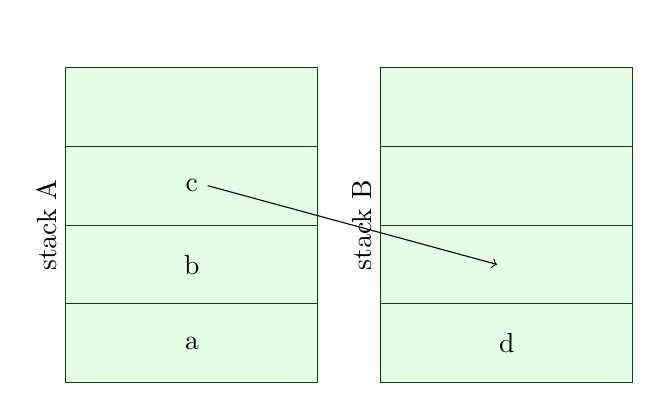
\begin{tikzpicture}

\drawstruct{(0,0)}
\structcell[freecell]{} \coordinate (Atm) at (currentcell.east);
\structcell[freecell]{}
\structcell[freecell] {} \coordinate (A) at (currentcell.west);
\structcell[freecell]{d} 
\structname{stack B
}

\drawstruct{(-4,0)}
\structcell[freecell]{} 
\structcell[freecell]{c} \coordinate (Btm) at (currentcell.east);
\structcell[freecell]{b}
\structcell[freecell]{a}
\structname{stack A}

\draw[->] (Btm) -- (A);

\end{tikzpicture}

push(A,pop(B));\\pop(B);

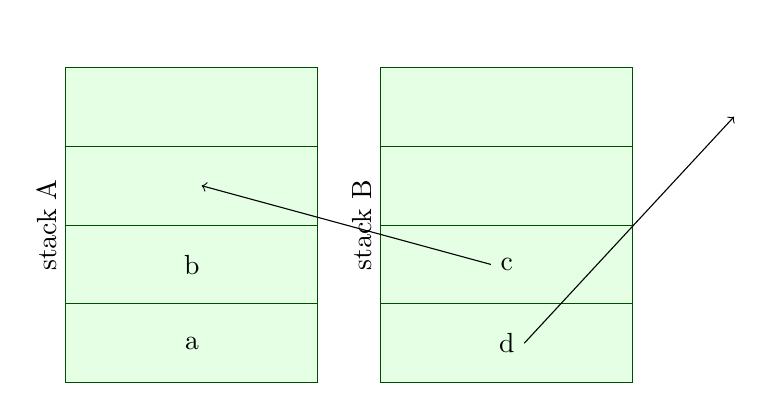
\begin{tikzpicture}
\draw (3, -1) node (Otm) {};
\drawstruct{(0,0)}
\structcell[freecell]{} 
\structcell[freecell]{}
\structcell[freecell] {c} \coordinate (A) at (currentcell.west);
\structcell[freecell]{d} \coordinate (Atm) at (currentcell.east); 
\structname{stack B
}

\drawstruct{(-4,0)}
\structcell[freecell]{} 
\structcell[freecell]{} \coordinate (Btm) at (currentcell.east);
\structcell[freecell]{b}
\structcell[freecell]{a}
\structname{stack A}

\draw[->] (A)   --   (Btm);
\draw[->]  (Atm) --  (Otm);

\end{tikzpicture}


\item 크기가 5인 배열로 구현된 스택 A에 다음과 같이 삽입과 삭제가 되풀이되었을 경우에 각 단계에서의 스택의 내용(1차원 배열의 내용, top의 값)을 나타내시오.

push(A,1);
\hspace{2cm}1
\begin{tabular}{|c|c|c|c|c|}
	\hline
	1&&&&\\
	\hline
\end{tabular}

push(A,2);
\hspace{2cm}2
\begin{tabular}{|c|c|c|c|c|}
	\hline
	1&2& & & \\
	\hline
\end{tabular}

push(A,3);
\hspace{2cm}3
\begin{tabular}{|c|c|c|c|c|}
	\hline
	1&2&3& & \\
	\hline
\end{tabular}

pop(A);
\hspace{2.5cm}2
\begin{tabular}{|c|c|c|c|c|}
	\hline
	1&2& & & \\
	\hline
\end{tabular}


push(A,4);
\hspace{2cm}3
\begin{tabular}{|c|c|c|c|c|}
	\hline
	1&2&4& & \\
	\hline
\end{tabular}

push(A,5);
\hspace{2cm}4
\begin{tabular}{|c|c|c|c|c|}
	\hline
	1&2&4&5& \\
	\hline
\end{tabular}

push(A,6);
\hspace{2cm}5
\begin{tabular}{|c|c|c|c|c|}
	\hline
	1&2&4&5&6\\
	\hline
\end{tabular}

push(A,7);
\hspace{2cm}5
\begin{tabular}{|c|c|c|c|c|}
	\hline
	1&2&4&5&6\\
	\hline
\end{tabular}

pop(A);
\hspace{2.5cm}4
\begin{tabular}{|c|c|c|c|c|}
	\hline
	1&2&4&5& \\
	\hline
\end{tabular}

\item 연결된 스택 A에 다음과 같이 삽입과 삭제가 되풀이되었을 경우에 각 단계에서의 연결된 스택의 내용(노드, top이 가리키는 값)을 나타내시오.

push(A,1);\hspace{2cm}1\\push(A,2);\hspace{2cm}2\\push(A,3);\hspace{2cm}3\\
pop(A);\hspace{2.5cm}2\\
push(A,5);\hspace{2cm}5\\push(A,6);\hspace{2cm}6\\pop(A);\hspace{2.5cm}5\\

\item 만약 연결된 스택의 C언어의 구현에서 만약 저장하려는 항목이 정수가 아니고 다음과 같은 구조체라면 소스의 어떤 부분들이 변경되어야 하는가?

\begin{lstlisting}[frame=none]
typedef struct {
	char name[MAX_NAME_SIZE];
	int student_no;
} element;
\end{lstlisting}
데이터 element에 맞게 삽입, 입력, 출력 부분을 바꾸어준다.

\item 괄호 검사 프로그램에서 다음의 입력을 처리한다고 가정할 때, 스택에 최대로 쌓이게 되는 괄호의 개수는 몇 개인가?

(([]\{\{\{\}\}\}))

5개

\item 알고리즘 5.1의 괄호 검사 프로그램에서 다음과 같은 수식이 주어졌을 경우, 알고리즘을 추적하여 각 단계에서의 스택의 내용을 그려라. 
\begin{enumerate}
	\item a{b[(c+d)*e]-f}
	\item {(a(b*c)/[d+e]/f)-g}
\end{enumerate}

\item 다음은 어떤 수식의 후위 표기이다. 이 때 최초로 수행되는 연산은 어느 것인가?

\begin{tabular}{|c|c|c|c|c|c|c|}
\hline
A&B&E&+&D&*&-\\
\hline
\end{tabular}

\begin{enumerate}
	\item B+E
	\item E+A
	\item D*B
	\item B*E
\end{enumerate}
	
\item 후위 표기식 계산 프로그램에서 다음과 같은 수식이 주어졌을 경우, 알고리즘을 추적하여 각 단계에서의 스택의 내용을 그려라. a=1, b=2, c=3, d=4, e=4라고 가정하라.
\begin{enumerate}
	\item ab*ca-/de*+
	\item ab-c*d+
\end{enumerate}

\item 배열로 구현된 스택에 저장된 요소의 수를 반환하는 size 연산을 구현하여 보라.
\begin{lstlisting}
int size(Stack* st) {
	return st->top;
}
\end{lstlisting}

\item 연결 리스트로 구현된 스택에 저장된 요소의 수를 반환하는 size 연산을 구현하여 보라.
\begin{lstlisting}
int size(Stack* st) {
	if(!st) return 0;
	return 1 + size(st->node);
}
\end{lstlisting}

\item 배열을 이용한 스택의 문제점은 스택을 생성할 때 MAX\_STACK\_SIZE를 결정해야 한다는 것이다.
이 결점을 보완하는 한 가지 방법은 max\_top이라는 변수를 도입하여 스택이 만들어질 때는 max\_top을 0으로 하여 시작하고 만약 삽입 연산 중에 새로운 요소를 추가할 공간이 없을 때에는, max\_top을 max\_top*2+1으로 변경하고 변경된 크기만큼의 공간을 동적으로 할당하여 새로운 배열을 만든다.
요소들은 이전 배열에서 새로운 배열로 복사되고 이전 배열은 지워진다.
비슷하게 만약 삭제 연산 중에 요소들의 개수가 배열 크기의 1/4로 떨어지게 되면 기존 크기의 절반인 배열을 생성하고 이전 요소들을 복사한 다음, 이전의 배열을 삭제한다.
이 스택을 구현하고 테스트하라.

\lstinputlisting{21.c}
\includegraphics[width=0.9\textwidth]{21.png}

\item 본문에는 단순 연결 리스트로 구현된 스택을 소개하였다. 4장 리스트에서 배운 이중 연결 리스트를 사용하여 연결된 스택을 구현하여 보라.
\end{enumerate}

\vspace{2cm}
{\Huge 소감}

리턴값을 잘 활용하면 리스트를 깔끔하게 만들 수 있다. 리스트는 재귀함수를 많이 활용할 수 있는 부분이었다. 포인터를 다루는 것은 아직도 많이 실수를 유발한다. 리스트를 좀 더 활용해 보기 위해 라인에디터를 직접 만들어 보았다. 라인을 삽입시에 개행문자가 하나 끼어드는 버그가 있다. 왜 그런지 잘 모르겠다. scanf를 fgets로 바꾸어 보기도 했는데 해결이 안된다.

\end{document}
